
\begin{frame}[t,allowframebreaks]{
    Momentum-based learning -}

    As the instantaneous direction of best movement is very rarely 
    the correct direction of descent, 
    \index{optimisation}\gls{optimisation} 
    often follows a zigzag trajectory.\\
    \vspace{0.2cm}
    \index{momentum}\Gls{momentum}-based methods \cite{Polyak:1964a}
    improve the  
    \index{gradient descent}\gls{gradient descent}, 
    by following an 
    {\bf {\em `averaged'} direction towards the minimum} 
    of the \index{loss function}\gls{loss function}.\\
    \begin{columns}
        \begin{column}{0.50\textwidth}
            \begin{center}
                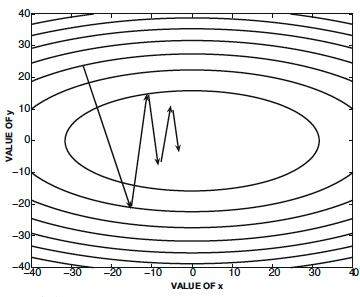
\includegraphics[width=0.98\textwidth]
                    {./images/training_issues/aggarwal18_shape_loss_function_grad_descent_R.png}\\
                {\tiny 
                    \color{col:attribution} 
                    Taken from Fig. 3.9 in \cite{Aggarwal:2018SpringerDL}.\\    
                }
            \end{center}                
        \end{column}
        \begin{column}{0.50\textwidth}
            \begin{itemize}
                \item
                The algorithm allows {\bf inertia}$^{1}$ 
                in the direction of descent.\\
                \begin{itemize}
                    \small
                    \item Builds inertia adding 
                    a new term to the parameter update rule.
                \end{itemize}
                \item
                The inertia helps to alleviate the amplitude 
                of oscillations from noisy 
                \index{gradient}\glspl{gradient}.\\
                \item
                By avoiding zigzagging, learning is accelerated.\\
            \end{itemize}
        \end{column}
    \end{columns}

    \framebreak

    %
    %
 
    In the plain \index{gradient descent}\gls{gradient descent}
    method, the parameter update is given by:
    \begin{equation}
        \vect{w}_{k} \rightarrow \vect{w}_{k+1} = 
            \vect{w}_{k} + \delta \vect{w}_{k} 
    \end{equation}\\
    where 
    \begin{equation}
        \delta \vect{w}_{k} = - \alpha \nabla_{\vect{w}} L(\vect{w}_{k})
    \end{equation}\\

    In the \index{momentum}\gls{momentum}-based method,
    the update rule is modified so that: 
    \begin{equation}
        \delta \vect{w}_{k} = 
          - \alpha \nabla_{\vect{w}} L(\vect{w}_{k})
          + \beta \delta \vect{w}_{k-1}
        \label{eq:momentum_method_update_rule}
    \end{equation}
    where $\beta$ $\in (0,1)$ is the 
    \index{momentum parameter}\gls{momentum parameter}.\\

    \vspace{0.2cm}

    Often, the step size, $\delta \vect{w}_{k}$, is referred to as the 
    \index{velocity}\gls{velocity},
    and the parameter $\beta$ as the 
    \index{friction parameter}\gls{friction parameter}.\\

    \framebreak

    %
    %

    As we've seen, in the \index{momentum}\gls{momentum}-based method,
    the update rule becomes: 
    \begin{equation*}
        \delta \vect{w}_{k} = 
          - \alpha \nabla_{\vect{w}} L(\vect{w}_{k})
          + \beta \delta \vect{w}_{k-1}
    \end{equation*}
    
    \begin{columns}[t]
        \begin{column}{0.60\textwidth}
            Larger values of 
            $\beta$, help to pick up a 
            \index{velocity}\gls{velocity} 
            towards the correct direction.\\
            \begin{center}
                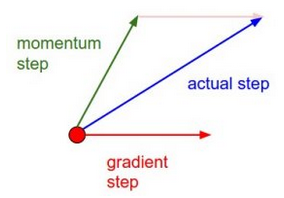
\includegraphics[width=0.50\textwidth]
                    {./images/training_issues/cs231n_momentum_update.png}\\
                {\tiny 
                    \color{col:attribution} 
                    Taken from \cite{CS231n}.\\    
                }
            \end{center}                
            The \gls{velocity} allows an effective 
            dumping of large sideways perturbations.\\        
        \end{column}
        \begin{column}{0.40\textwidth}
            \vspace{-0.5cm}
            \begin{center}
                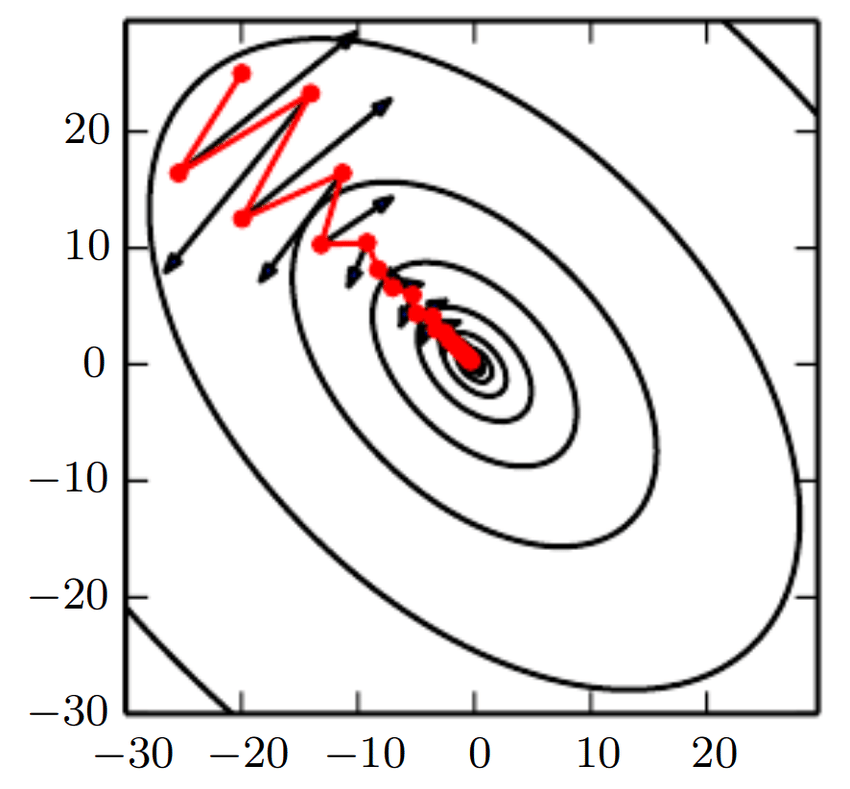
\includegraphics[width=0.98\textwidth]
                    {./images/training_issues/goodfellow17_search_path_w_momentum.png}\\
                {\scriptsize
                  Black: \index{gradient}\gls{gradient} step.
                  Red: actual step of \gls{momentum}-based method.\\
                }
                {\tiny 
                    \color{col:attribution} 
                    Taken from Fig. 8.5 in \cite{Goodfellow:2017MITDL}.\\    
                }
            \end{center}                
        \end{column}
    \end{columns}

    \framebreak

    %
    %

    The \index{momentum}\gls{momentum}-based methods {\bf overshoot} in 
    the direction of \index{velocity}\gls{velocity}.
    \begin{itemize}
        \small
        \item Similarly as a ball rolling down a bowl will overshoot the minimum.
    \end{itemize}    
    \vspace{0.1cm}
    Nevertheless, \gls{momentum}-based methods perform better.
    \begin{itemize}
        \small
        \item Faster approach to the minimum
        more than compensates for overshooting.
    \end{itemize}    
    \vspace{0.1cm}
    Overshooting can be beneficial to the extend it helps escape local minima.\\

    \begin{center}
        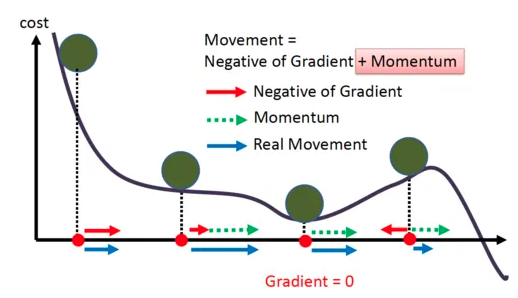
\includegraphics[width=0.60\textwidth]
            {./images/training_issues/khandewal20_gradient_descent_ball.png}\\
        {\tiny 
            \color{col:attribution} 
            Taken from \cite{Medium:GradDescentMomRMSPropAdam}.\\    
        }
    \end{center}                        

    \framebreak

    %
    %

    To elucidate the previous formulas, study the following pseudo-code.\\
    \vspace{0.1cm}
    \begin{block}{
        Mini-batch \index{gradient descent}\gls{gradient descent}
        with \index{momentum}\gls{momentum}}
    {\tt \scriptsize
       {\bf Set} hyperparameters 
       (learning rate $\alpha$, momentum parameter $\beta$) to desired values\\
       \vspace{0.1cm}
       {\bf Randomize} initial set of network weights, $\vect{w}_{0}$\\
       \vspace{0.1cm}
       {\bf Initialize} auxiliary variables: $k=-1$, $\delta \vect{w}_{-1} = 0$\\
       \vspace{0.1cm}
       {\bf While} [convergence condition not met]:\\
       \vspace{0.1cm}
       \begin{itemize}        
        {\scriptsize
        \item Increment $k$
        \vspace{0.2cm}
        \item Sample a minibatch of $N$ training examples 
        $(\vect{x}_i, y_i)$
        \item Compute the loss gradient:
        $\displaystyle g_k = \frac{1}{N} \nabla_{\vect{w}} 
          \sum_{i=0}^{N-1} L\Big(f(\vect{x}_i, \vect{w}_{k}),y_i\Big)$ 
        \item Compute the velocity update: $\delta \vect{w}_{k} =  
                - \alpha g_k
                + \beta \delta \vect{w}_{k-1}$\\
        \vspace{0.2cm}
        \item Apply the update to the network parameters: 
              $\vect{w}_{k+1} = \vect{w}_{k} + \delta \vect{w}_{k}$
        }
       \end{itemize}
       {\bf End while}
    }
    \end{block}

    \framebreak

    %
    %

    Following the first few steps of the algorithm, 
    we find for the {\em velocity}:

    \begin{equation*}
        \delta \vect{w}_{0} = 
        - \alpha \nabla_{\vect{w}} L(\vect{w}_{0})
        + \beta \cancelto{0}{\delta \vect{w}_{-1}}
    \end{equation*}

    \vspace{-0.1cm}

    \begin{equation*}
        \delta \vect{w}_{1} = 
        - \alpha \nabla_{\vect{w}} L(\vect{w}_{1})
        + \beta \delta \vect{w}_{0} =
        - \alpha \Big(
            \nabla_{\vect{w}} L(\vect{w}_{1}) +
            \beta \nabla_{\vect{w}} L(\vect{w}_{0})
        \Big)
    \end{equation*}

    \vspace{-0.4cm}

    \begin{equation*}
        \delta \vect{w}_{2} = 
        - \alpha \nabla_{\vect{w}} L(\vect{w}_{2})
        + \beta \delta \vect{w}_{1} = %\Rightarrow
        - \alpha \Big(
            \nabla_{\vect{w}} L(\vect{w}_{2}) +
            \beta \nabla_{\vect{w}} L(\vect{w}_{1}) +
            \beta^2 \nabla_{\vect{w}} L(\vect{w}_{0})
        \Big)
    \end{equation*}

    \begin{equation*}
        \cdots
    \end{equation*}

    \vspace{0.1cm}

    This generalizes to:\\

    \vspace{-0.4cm}

    \begin{equation}
        \frac{-\delta \vect{w}_{k}}{\alpha} = 
            \nabla_{\vect{w}} L(\vect{w}_{k}) +
            \beta \nabla_{\vect{w}} L(\vect{w}_{k-1}) +
            \beta^2 \nabla_{\vect{w}} L(\vect{w}_{k-2}) + 
            \cdots + 
            \beta^k \nabla_{\vect{w}} L(\vect{w}_{0}) 
        \label{eq:grad_descent_momentum_step_k}
    \end{equation}

    \framebreak

    %
    %

    As we observe from Eq.~\ref{eq:grad_descent_momentum_step_k}
    \begin{equation*}
        \frac{-\delta \vect{w}_{k}}{\alpha} = 
            \nabla_{\vect{w}} L(\vect{w}_{k}) +
            \beta \nabla_{\vect{w}} L(\vect{w}_{k-1}) +
            \beta^2 \nabla_{\vect{w}} L(\vect{w}_{k-2}) + 
            \cdots + 
            \beta^k \nabla_{\vect{w}} L(\vect{w}_{0}) 
    \end{equation*}

    the \index{velocity}\gls{velocity} 
    $\delta \vect{w}_{k}$ {\bf accumulates \index{gradient}\glspl{gradient}}.

    \vspace{0.2cm}

    \Glspl{gradient} from further back in the past of the 
    \index{optimisation}\gls{optimisation} process, 
    are weighted with a higher power of 
    the \index{momentum parameter}\gls{momentum parameter} $\beta$ ($\in (0,1)$).

    \vspace{0.2cm}

    The \gls{velocity} $\delta \vect{w}_{k}$ is an 
    {\bf exponentially decaying moving average of past gradients}.

    \framebreak

    %
    %

    We note that the step depends on the size 
    and {\bf alignment} of the gradients.\\
    \vspace{0.2cm}

    If the code observed a constant gradient $\vect{g}$, 
    Eq. \ref{eq:grad_descent_momentum_step_k} becomes:\\
    \begin{equation}
        \delta \vect{w}_{k} = 
            -\alpha \vect{g} \Big(
               1 + \beta + \beta^2 + \cdots + \beta^k
            \Big)
    \end{equation}

    Above, we recognise a geometric series 
    written in closed form as:\\
    \begin{equation}
        1 + \beta + \beta^2 + \cdots + \beta^k = \frac{1}{1-\beta}
    \end{equation}

    Therefore, the velocity reaches a {\em terminal} value of:\\
    \begin{equation}
        \delta \vect{w}_{k} = 
            \frac{-\alpha \vect{g}}{1-\beta} \Rightarrow
        |\delta \vect{w}_{k}| = 
            \frac{\alpha |\vect{g}|}{1-\beta} 
    \end{equation}

    \vspace{0.1cm}

    For $\beta$=0.9, 
    the typical gradient descent step, $\alpha |\vect{g}|$,
    for this situation,
    is increased by a factor $1/(1-\beta)$=10.\\
    % \vspace{0.1cm}
    % \noindent\rule{4cm}{0.4pt}\\
    % {\scriptsize
    % $^{(1)}$ For $|r|<$1, $\displaystyle \sum_{k=0}^{\infty}ar^k = \frac{a}{1-r}$.
    % }

\end{frame}

